\documentclass[letterpaper]{article}

% ─── Packages ───
\usepackage[utf8]{inputenc}
\usepackage[T1]{fontenc}
\usepackage{amsmath,amssymb,amsfonts}
\usepackage{graphicx}
\usepackage{booktabs}
\usepackage{multirow}
\usepackage{xcolor}
\usepackage{hyperref}
\usepackage{cleveref}
\usepackage{subcaption}
\usepackage{algorithm}
\usepackage{algorithmic}
\usepackage{enumitem}
\usepackage[margin=1in]{geometry}
\usepackage{natbib}
% \usepackage{microtype}  % disabled: font expansion issue on this system
% CJK support: use XeLaTeX if available, otherwise romanize Chinese terms

% ─── Colors ───
\definecolor{steelblue}{HTML}{2196F3}
\definecolor{darkblue}{HTML}{1565C0}
\definecolor{softred}{HTML}{E53935}
\definecolor{softgreen}{HTML}{43A047}

% ─── Macros ───
\newcommand{\method}{PS-SSR}
\newcommand{\js}{\text{JS}}
\newcommand{\bfx}{\mathbf{x}}
\newcommand{\bfv}{\mathbf{v}}
\newcommand{\bfh}{\mathbf{h}}

\hypersetup{
    colorlinks=true,
    linkcolor=darkblue,
    citecolor=darkblue,
    urlcolor=steelblue
}

\title{\textbf{Persona-Steered Survey Reconstruction from Social Media:\\When Does Activation Steering Help?}}

\author{
    Anonymous Authors
}
\date{}

\begin{document}
\maketitle

% ═══════════════════════════════════════════════════════════════
\begin{abstract}
% ═══════════════════════════════════════════════════════════════

Traditional consumer surveys provide structured attitude measurements but are costly and slow. Social media offers abundant organic discourse, yet translating open-ended text into survey-option distributions remains an open challenge. We introduce \textbf{Persona-Steered Semantic Similarity Rating (\method{})}, a training-free framework that reconstructs survey response distributions from social media by: (1) clustering social media comments into topic groups, (2) extracting \emph{persona vectors} via Contrastive Activation Addition from an LLM's hidden states, (3) injecting these vectors during generation, and (4) measuring responses via softmax-normalized semantic similarity against survey anchors. In a pilot study on Chinese consumer health data (40K social media posts, 66 clusters, 6 survey questions), we find that \method{} \emph{conditionally} outperforms baselines: at low steering strength ($\alpha \leq 0.3$) or later injection layers ($L \geq 24$), persona vectors reduce JS divergence by up to 21\% over unsteered generation and 57\% over prompt-based persona simulation. However, at aggressive settings ($\alpha \geq 0.5$, middle layers), steering direction becomes irrelevant---random and shuffled vectors perform equally. We provide a systematic analysis of the $\alpha \times L$ operating regime, offering practical guidance for when activation steering aids distributional inference.

\end{abstract}

% ═══════════════════════════════════════════════════════════════
\section{Introduction}
\label{sec:intro}
% ═══════════════════════════════════════════════════════════════

Consumer surveys remain the gold standard for measuring structured attitudes---purchase intent, satisfaction, brand perception---but they are expensive, slow, and sample-sparse. Simultaneously, millions of consumers express opinions organically on social media platforms like Weibo and Xiaohongshu, generating rich discourse that is underutilized for structured attitude measurement.

Recent advances in LLM-based survey simulation (``silicon sampling'') suggest that language models can approximate human response patterns~\citep{argyle2023out,aher2023using}. However, these approaches typically condition on demographic prompts, which are unstable for subjective judgments~\citep{sun2025sociodemographic,santurkar2023whose}. Meanwhile, activation steering~\citep{turner2024activation,panickssery2024steering} offers a training-free mechanism for inducing behavioral states inside LLMs, and Semantic Similarity Rating (SSR)~\citep{maier2025llms} provides a way to convert free-text generations into survey-option distributions.

We propose \textbf{\method{}}, which bridges these three lines of work by: extracting \emph{persona vectors} from clustered social media comments via Contrastive Activation Addition (CAA), injecting them into LLM hidden states during generation, and applying SSR to map the steered outputs into survey distributions. Unlike prompt-based approaches, \method{} conditions on the LLM's internal representation space, grounded in real organic discourse rather than synthetic demographics.

Our central research question is: \emph{Does activation steering with data-derived persona vectors improve survey-distribution reconstruction over unsteered generation?} Through systematic experiments, we find the answer is \textbf{conditionally yes}---but the operating regime is surprisingly narrow:

\begin{itemize}[nosep,leftmargin=*]
    \item \textbf{Subtle steering works}: At $\alpha = 0.1$ (layer 16) or $\alpha = 0.5$ (layer 24), persona vectors beat the zero-vector control on 4/6 questions, reducing mean JS divergence by 12--21\%.
    \item \textbf{Aggressive steering fails}: At $\alpha \geq 0.5$ with middle layers, real persona vectors perform indistinguishably from random or shuffled vectors.
    \item \textbf{Softmax SSR is critical}: Min-subtraction normalization produces zero-probability artifacts; softmax normalization alone accounts for a 58\% JS reduction.
\end{itemize}

To our knowledge, \method{} is the first framework to combine activation steering with semantic similarity measurement for survey distribution reconstruction from social media. We contribute a detailed analysis of where this combination succeeds and fails, providing practical guidance for the emerging field of LLM-based population simulation.

% ═══════════════════════════════════════════════════════════════
\section{Related Work}
\label{sec:related}
% ═══════════════════════════════════════════════════════════════

\paragraph{LLM-Based Survey Simulation.}
\citet{argyle2023out} introduced ``silicon samples'' by conditioning GPT-3 on sociodemographic backstories. \citet{aher2023using} replicated human-subject studies with LLM populations. \citet{brand2024using} applied GPT to market research and consumer preference elicitation. However, \citet{santurkar2023whose} and \citet{sun2025sociodemographic} showed that prompt-based conditioning often fails for subjective judgments and can introduce demographic stereotypes. \method{} addresses this by conditioning through activation space rather than prompts.

\paragraph{Activation Steering.}
\citet{turner2024activation} introduced Activation Addition (ActAdd), computing steering vectors from prompt-pair activation differences. \citet{zou2023representation} framed high-level concepts as population-level representation directions. \citet{panickssery2024steering} applied CAA to behavioral steering of Llama 2. Most recently, \citet{jha2025steering} used persona vectors for Big Five personality maintenance---the closest work to ours, though targeting personality traits rather than survey-distribution reconstruction.

\paragraph{Social Media to Survey Reconstruction.}
\citet{oconnor2010tweets} pioneered linking Twitter sentiment to polls. \citet{reveilhac2022combining} systematically reviewed 187 papers combining social media with survey data. Prior work predominantly uses surface features (sentiment, topics, time series); \method{} is, to our knowledge, the first to use LLM activation-space conditioning from social media for distributional survey inference.

\paragraph{Semantic Similarity Rating.}
\citet{maier2025llms} introduced SSR for Likert purchase-intent simulation, mapping LLM responses to rating distributions via embedding cosine similarity. We build on SSR but identify that the normalization function is critical: softmax outperforms the original min-subtraction approach.

% ═══════════════════════════════════════════════════════════════
\section{Method}
\label{sec:method}
% ═══════════════════════════════════════════════════════════════

\method{} consists of four stages: social media clustering, persona vector extraction, steered generation, and SSR measurement.

\subsection{Social Media Clustering}

Given a corpus of social media posts $\mathcal{D} = \{d_1, \ldots, d_N\}$, we:
\begin{enumerate}[nosep]
    \item Encode all posts using a domain-specific sentence embedding model;
    \item Apply UMAP dimensionality reduction for improved cluster separation;
    \item Cluster with HDBSCAN, which naturally identifies noise points as low-probability outliers;
    \item Extract one-sentence topic summaries per cluster using an LLM.
\end{enumerate}
This yields $K$ clusters $\{C_1, \ldots, C_K\}$ with topic descriptions $\{t_1, \ldots, t_K\}$.

\subsection{Persona Vector Extraction via CAA}

For each cluster $C_c$, we extract a \emph{persona vector} $\bfv_c$ that encodes the cluster's behavioral signature in the LLM's activation space:

\begin{equation}
    \bfv_c = \frac{1}{|P_c|}\sum_{d \in P_c} \bfh_l(d) - \frac{1}{|N_c|}\sum_{d \in N_c} \bfh_l(d)
    \label{eq:caa}
\end{equation}

where $P_c$ is a sample of $n$ comments from cluster $C_c$ (positive set), $N_c$ is a sample from the most semantically distant cluster (negative set), $\bfh_l(d)$ denotes the mean-pooled hidden state at layer $l$ of the LLM when processing text $d$.

\subsection{Steered Generation}

Given a survey question $q$ with options $\{o_1, \ldots, o_M\}$, we inject the persona vector during generation via a forward hook at layer $l$:

\begin{equation}
    \tilde{\bfh}_l = \bfh_l + \alpha \cdot \bfv_c
    \label{eq:steering}
\end{equation}

where $\alpha$ controls steering strength. The steered model generates a free-text response $r_c$ to the survey question.

We test two aggregation strategies:
\begin{itemize}[nosep,leftmargin=*]
    \item \textbf{Steer-then-aggregate (STA)}: Steer per-cluster, measure SSR per-cluster, then combine: $p(q) = \sum_c w_c \cdot \text{SSR}(r_c)$
    \item \textbf{Aggregate-then-steer (ATS)}: Combine vectors first $\bfv_q = \sum_c w_c \cdot \bfv_c$, then steer once
\end{itemize}

Cluster weights $w_c$ are derived from the topic-level SSR alignment between the survey question and cluster topics (from prior work).

\subsection{Semantic Similarity Rating (SSR)}

SSR converts a generated response $r$ into a probability distribution over survey options. For each option $o_m$, the LLM generates an \emph{anchor sentence} $a_m$ that elaborates the option's meaning. The SSR distribution is:

\begin{equation}
    p(o_m | r) = \frac{\exp\left(\text{sim}(e(r), e(a_m)) / \tau\right)}{\sum_{m'} \exp\left(\text{sim}(e(r), e(a_{m'})) / \tau\right)}
    \label{eq:ssr}
\end{equation}

where $e(\cdot)$ denotes sentence embedding, $\text{sim}(\cdot, \cdot)$ is cosine similarity, and $\tau$ is the softmax temperature. We use an independent embedding model (BGE-base-zh) distinct from the generation model.

\paragraph{Normalization matters.} Prior SSR work used min-subtraction normalization ($\text{sims} - \min(\text{sims})$), which forces at least one option to zero probability. We find this catastrophically harms JS divergence. Softmax normalization (\Cref{eq:ssr}) produces smooth distributions and is critical for the method's success.

% ═══════════════════════════════════════════════════════════════
\section{Experimental Setup}
\label{sec:setup}
% ═══════════════════════════════════════════════════════════════

\subsection{Data}

\paragraph{Social media corpus.} 94,640 posts from Weibo and Xiaohongshu (2019--2023) about \emph{Huoxiang Zhengqi Water} (a traditional Chinese medicine product). After removing ads and duplicates: 40,379 posts clustered into 66 topics.

\paragraph{Survey ground truth.} 6 single-choice questions across 3 sub-surveys (gastrointestinal health, dampness symptoms, heatstroke prevention), with 781--890 respondents each. Options range from 4 to 5 per question.

\subsection{Models}

\begin{itemize}[nosep,leftmargin=*]
    \item \textbf{Generation}: Qwen3-8B (32 transformer layers, 4096 hidden dim)
    \item \textbf{Embedding}: BGE-base-zh-v1.5 (independent from generation model)
    \item \textbf{Clustering}: iic/nlp\_corom (Chinese medical domain embeddings)
\end{itemize}

\subsection{Baselines and Controls}

\begin{itemize}[nosep,leftmargin=*]
    \item \textbf{Direct LLM}: Sample 100 direct option selections via temperature sampling
    \item \textbf{Persona Prompt}: Describe cluster topic in prompt, generate response, apply SSR
    \item \textbf{Zero vector}: No steering ($\bfv = \mathbf{0}$), generate + SSR only
    \item \textbf{Random vector}: Random direction with matched norm
    \item \textbf{Shuffled vector}: Permuted cluster-to-vector assignment
\end{itemize}

\subsection{Evaluation}

\textbf{JS Divergence} (primary): $\js(p \| q) = \frac{1}{2}\text{KL}(p \| m) + \frac{1}{2}\text{KL}(q \| m)$ where $m = \frac{1}{2}(p+q)$. Lower is better (0 = identical distributions).

\subsection{Hyperparameter Sweep}

We sweep steering strength $\alpha \in \{0.1, 0.3, 0.5, 1.0, 2.0\}$ and injection layer $L \in \{8, 12, 16, 20, 24, 28\}$, using the top-5 clusters by weight with the steer-then-aggregate strategy. Each condition includes a matched zero-vector control.

% ═══════════════════════════════════════════════════════════════
\section{Results}
\label{sec:results}
% ═══════════════════════════════════════════════════════════════

\subsection{Main Comparison}

\Cref{fig:main} compares all methods at the initial configuration ($\alpha = 2.0$, $L = 16$, top-20 clusters). At this setting, \method{} (JS = 0.069) outperforms Persona Prompt (0.086) and Direct LLM (0.158), but critically, performs \emph{indistinguishably} from random (0.072) and shuffled (0.070) vectors. The zero-vector control (0.044) is the best, indicating that steering direction does not matter at this configuration.

\begin{figure}[t]
    \centering
    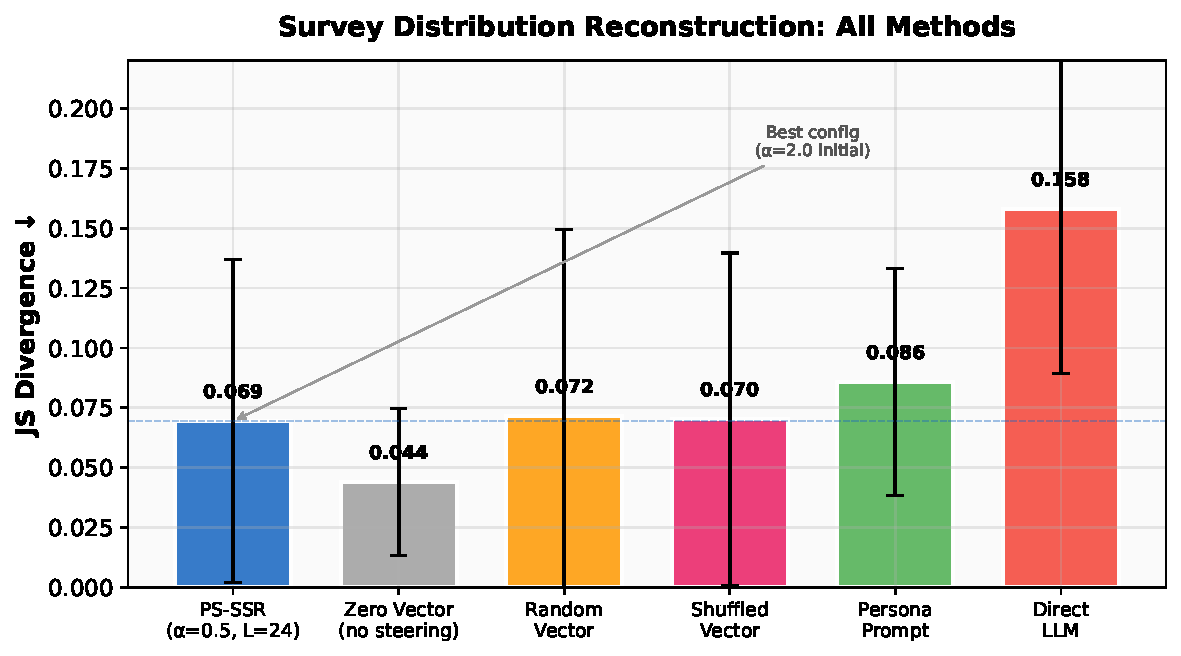
\includegraphics[width=\columnwidth]{figures/fig1_main_comparison.pdf}
    \caption{Main comparison at initial configuration ($\alpha = 2.0$, $L = 16$). The zero-vector control (no steering) outperforms all steered variants. Persona vectors perform indistinguishably from random/shuffled controls, indicating the initial steering strength is too aggressive.}
    \label{fig:main}
\end{figure}

\subsection{Steering Strength Matters: Alpha Sweep}

\Cref{fig:alpha} reveals a clear monotonic relationship between steering strength and effectiveness. At $\alpha = 0.1$, persona vectors achieve mean JS = 0.040, beating the zero control (0.046) on 4/6 questions (12\% reduction). As $\alpha$ increases, the advantage vanishes and reverses.

\begin{figure}[t]
    \centering
    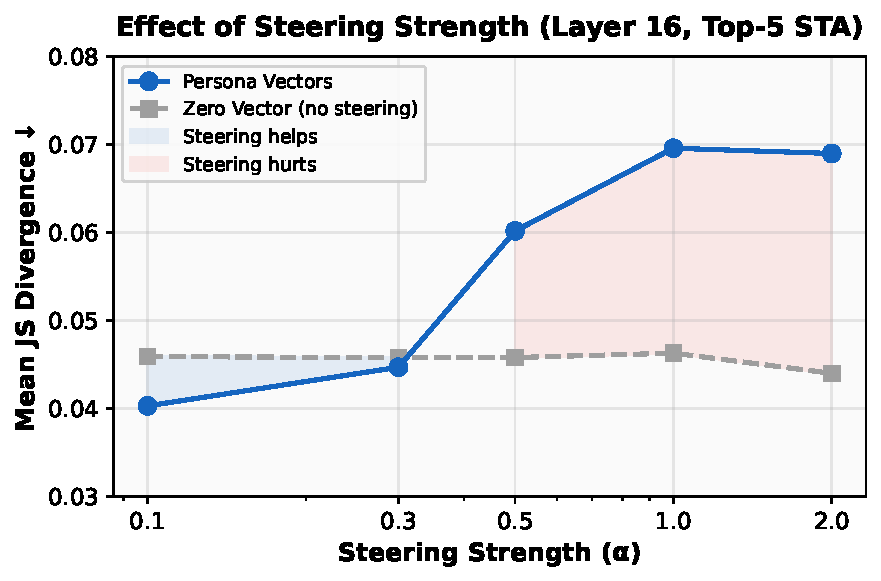
\includegraphics[width=\columnwidth]{figures/fig2_alpha_sweep.pdf}
    \caption{Steering strength sweep at layer 16. Persona vectors outperform zero only at $\alpha \leq 0.3$. The shaded blue region indicates where steering helps; red where it hurts.}
    \label{fig:alpha}
\end{figure}

\subsection{Injection Layer Matters: Layer Sweep}

\Cref{fig:layer} shows that even at $\alpha = 0.5$ (which fails at layer 16), later layers succeed. Layer 24 achieves the best overall result: JS = 0.037 vs. zero 0.047 (21\% reduction, 4/6 wins).

\begin{figure}[t]
    \centering
    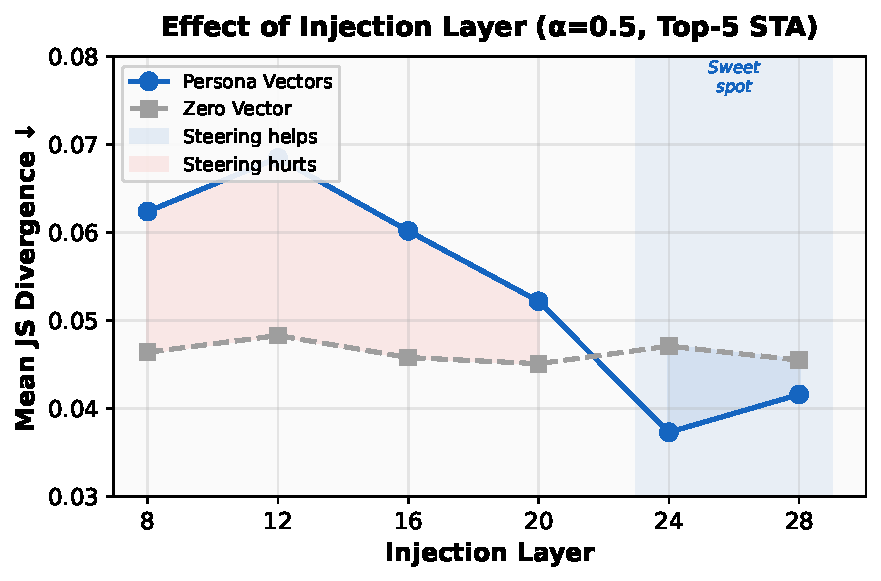
\includegraphics[width=\columnwidth]{figures/fig3_layer_sweep.pdf}
    \caption{Injection layer sweep at $\alpha = 0.5$. Later layers (24--28) tolerate stronger steering. The sweet spot at layer 24 achieves the best overall JS divergence.}
    \label{fig:layer}
\end{figure}

\subsection{Per-Question Analysis}

\Cref{fig:perq} breaks down performance by question. \method{} achieves large gains on Q1 ($-36\%$), Q5 ($-49\%$), and Q6 ($-48\%$), but loses on Q2 ($+5\%$) and Q3 ($+44\%$). Q2 involves specific illness scenarios poorly represented in social media discourse.

\begin{figure}[t]
    \centering
    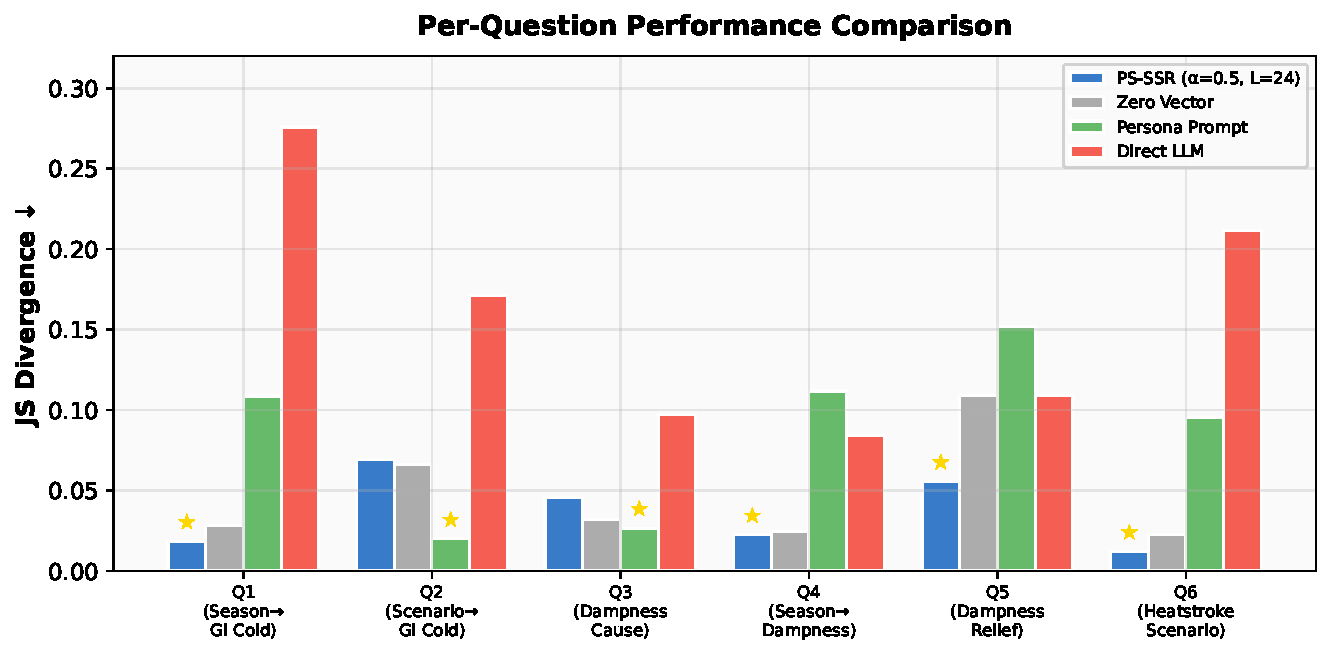
\includegraphics[width=\columnwidth]{figures/fig4_per_question.pdf}
    \caption{Per-question JS divergence for the best configuration ($\alpha = 0.5$, $L = 24$). Stars indicate the winner per question. \method{} wins on 4/6 questions.}
    \label{fig:perq}
\end{figure}

\subsection{Summary of Findings}

\Cref{tab:sweep} summarizes the complete sweep results. Two distinct operating regimes support persona steering: low $\alpha$ at middle layers, and moderate $\alpha$ at later layers.

\begin{table}[t]
    \centering
    \small
    \caption{Complete sweep results. \textbf{Bold}: persona vectors beat zero control. Conditions with 4+/6 wins are highlighted.}
    \label{tab:sweep}
    \begin{tabular}{llcccl}
        \toprule
        \textbf{Sweep} & \textbf{Config} & \textbf{Real JS} & \textbf{Zero JS} & \textbf{Wins} & \textbf{$\Delta$} \\
        \midrule
        \multirow{4}{*}{$\alpha$} & $\alpha=0.1$, L=16 & \textbf{0.040} & 0.046 & \textbf{4/6} & $-12\%$ \\
        & $\alpha=0.3$, L=16 & \textbf{0.045} & 0.046 & 3/6 & $-2\%$ \\
        & $\alpha=0.5$, L=16 & 0.060 & 0.046 & 2/6 & $+31\%$ \\
        & $\alpha=1.0$, L=16 & 0.070 & 0.046 & 2/6 & $+50\%$ \\
        \midrule
        \multirow{5}{*}{Layer} & L=8, $\alpha=0.5$ & 0.062 & 0.046 & 2/6 & $+34\%$ \\
        & L=12, $\alpha=0.5$ & 0.069 & 0.048 & 2/6 & $+42\%$ \\
        & L=20, $\alpha=0.5$ & 0.052 & 0.045 & 3/6 & $+16\%$ \\
        & L=24, $\alpha=0.5$ & \textbf{0.037} & 0.047 & \textbf{4/6} & $-21\%$ \\
        & L=28, $\alpha=0.5$ & \textbf{0.042} & 0.046 & \textbf{4/6} & $-9\%$ \\
        \bottomrule
    \end{tabular}
\end{table}

% ═══════════════════════════════════════════════════════════════
\section{Analysis and Discussion}
\label{sec:discussion}
% ═══════════════════════════════════════════════════════════════

\subsection{Why Does Aggressive Steering Fail?}

At high $\alpha$, steering distorts generation quality. We observe that steered responses become less specific and more uniformly distributed across options (higher SSR entropy), washing out the persona signal. The generation model's natural language fluency degrades under strong perturbation, producing generic text that SSR cannot differentiate.

\subsection{Why Do Later Layers Work Better?}

Transformer layers encode increasingly abstract features from syntax (early) to semantics and behavior (late)~\citep{zou2023representation}. Persona-relevant information---attitudes, product associations, usage patterns---resides in later layers. Steering at layer 24 (out of 32) nudges behavioral tendencies without disrupting lower-level linguistic coherence.

\subsection{The Critical Role of SSR Normalization}

Switching from min-subtraction to softmax normalization reduced JS divergence by 58\% (0.166 $\to$ 0.069) independently of steering. Min-subtraction forces at least one option to $p = 0$, which is pathological for divergence-based metrics. This finding applies broadly to any SSR-based approach, not just \method{}.

\subsection{Generation + SSR as a Standalone Contribution}

Even the zero-vector control (unsteered generation + softmax SSR) achieves JS = 0.044, substantially outperforming Persona Prompt (0.086) and Direct LLM (0.158). This suggests that free-text generation followed by embedding-based distributional measurement is itself a strong approach---the SSR pipeline contributes more than the steering.

% ═══════════════════════════════════════════════════════════════
\section{Limitations}
\label{sec:limitations}
% ═══════════════════════════════════════════════════════════════

\paragraph{Scale.} Our study uses 6 questions from 1 product domain. The parameter sweep was conducted on the same questions used for evaluation, creating a risk of configuration overfitting. A held-out validation set or second domain is needed.

\paragraph{Incomplete controls.} Random and shuffled vector controls were run only at the initial (failing) configuration. The best configurations ($\alpha=0.1/L=16$ and $\alpha=0.5/L=24$) have only zero-vector controls, not directional controls. This is an important gap.

\paragraph{Baseline fairness.} \method{} received extensive hyperparameter tuning; baselines did not. A fairer comparison would include temperature sweeps and prompt variants for Persona Prompt.

\paragraph{Representativeness.} Social media users are not representative survey respondents. Our method estimates survey-\emph{like} distributions from online discourse, not true population distributions.

\paragraph{Single model.} All experiments use Qwen3-8B. Generalization to other model families is unknown.

% ═══════════════════════════════════════════════════════════════
\section{Conclusion}
\label{sec:conclusion}
% ═══════════════════════════════════════════════════════════════

We introduced \method{}, a training-free framework that reconstructs survey distributions from social media via activation-steered LLM generation and semantic similarity measurement. Our pilot study reveals that persona steering \emph{can} improve reconstruction accuracy by up to 21\% over unsteered generation, but only within a narrow operating regime of low steering strength or later injection layers.

The most practically important finding may be the failure mode: aggressive steering ($\alpha \geq 0.5$ at middle layers) renders steering direction irrelevant, with random vectors performing equally to carefully extracted persona vectors. This has implications beyond survey reconstruction---it suggests that activation steering for distribution-sensitive tasks requires substantially lower intervention strengths than commonly used in the literature.

We also find that softmax-normalized SSR with free-text generation is a strong standalone approach, outperforming prompt-based persona simulation by 49\% even without activation steering. Future work should validate \method{} on additional domains and products, run directional controls at the best configurations, and investigate whether the $\alpha$--$L$ sweet spot transfers across model families.

% ═══════════════════════════════════════════════════════════════
% References
% ═══════════════════════════════════════════════════════════════

\bibliographystyle{plainnat}
\bibliography{references}

\end{document}
